% !TEX root = ../report.tex
\section{Das Graphical User Interface} \label{GUISec}
\begin{Spacing}{\mylinespace}

Zur Interaktion und Einstellung der einzelnen Komponenten entschieden wir uns dafür, unserer Anwendung ein \textit{Graphical User Interface} (GUI) zu spendieren. 

\subsection{Die Anforderungen}

Als Anforderungen setzten wir uns ein übersichtliches und leicht verständliches System, welches uns im Laufe des Projekts ermöglichen sollte, schnell und ohne größeren Aufwand, neue Funktionalitäten hinzuzufügen.  

\subsection{Die Umsetzung}

Um diese Anforderungen zu erreichen experimentierten wir im ersten Projektsemester mit einem \textit{Multi-Window} Ansatz auf Basis von \textit{Windows Forms}. Dieser Ansatz bestand aus zwei separaten Fenstern (s. Abbildung \ref{fig:GUIOld}). Ein Fenster, das für die Projektion auf den Sand, mit Hilfe des Beamers genutzt wurde und ein weiteres Fenster für die 3D-Ansicht, Zusatzinformationen und den Bedienelementen zur Anpassung des Systems.
\\\\
Leider stellte sich recht schnell heraus, dass dieser Ansatz doch nicht ganz so flexibel war, wie anfangs erwartet und das hinzufügen von neuen Bedienelementen jedes Mal mit relative viel Arbeit verbunden war. Zudem bedeuteten die beiden Fenster auch die doppelte Arbeit, da die komplette Szene jeweils zweimal gezeichnet werden musste. Aus diesen Gründen, entschlossen wir uns zu Beginn des zweiten Projektsemesters, diesen Ansatz zu verwerfen und auf ein einzelnes Fenster mit einer GPU-basierten GUI zu setzen.

\begin{figure}[h!]
	\centering
	\vspace*{30px}
	\includegraphics[width=320px]{graphics/gui.png}	
	\caption{Multi-Window GUI aus dem ersten Projektsemester.}
	\label{fig:GUIOld}
\end{figure}

\begin{description}
	\item[Ruminate GUI] \hfill \\
	Nach längerer Recherche und Suche nach einer passenden Bibliothek zur Darstellung eines GUI unter XNA, entschieden wir uns letztendlich für die sehr minimalistische, Open-Source Bibliothek \textit{Ruminate} \cite{Fra13}. Diese bot uns grundlegende Bedienelemente (s. Abbildung \ref{fig:Ruminate}) wie Buttons, Slider, usw. und war weitaus weniger überladen als die meisten anderen Bibliotheken.
\\\\
Natürlich hatte auch diese Bibliothek nicht nur Vorteile. Da diese von einem Ein-Mann-Team als Hobbyprojekt entwickelt wurde, gab es hier und da noch das ein oder andere Problem und auch das Design der Bedienelemente war nicht das schönste. Dank Open-Source, konnten wir uns aber selbst um diese Probleme kümmern und das GUI individuell an unser System anpassen.
	
\begin{figure}[h!]
	\centering
	\vspace*{20px}
	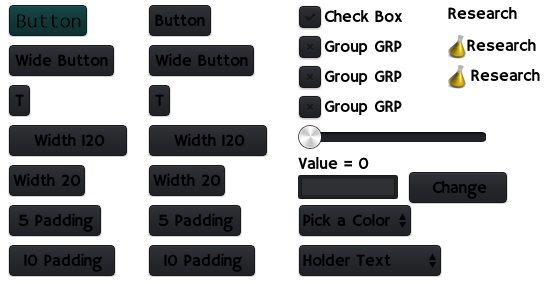
\includegraphics[width=250px]{graphics/ruminate.png}	
	\caption{Einige Bedienelemente der Ruminate GUI \cite{Fra13}.}
	\label{fig:Ruminate}
\end{figure}
	
	\item[Reflections] \hfill \\
	Um das Problem, mit dem sehr unflexiblen und statischen hinzufügen einzelner Bedienelementen pro konfigurierbarer Eigenschaft zu beheben, nutzten wir sogenannte \textit{Reflections}. Diese erlauben es zur Laufzeit auf die Struktur (Name, Typ, Methoden, Properties, usw.) eines gegebenen Objekts zuzugreifen und diese zu manipulieren. Mit dieser Technik konnten wir nun unser einzelnen \textit{Component Properties} (s. Abschnitt \ref{PropSec}), an die GUI Komponente übergeben und auf deren Typ und die einzelnen konfigurierbaren Eigenschaften zugreifen. Mit diesen Informationen konnte nun ein voll dynamisches GUI konstruiert werden (s. Abbildung \ref{fig:GUIReflect}). Sobald nun einer der \textit{Component Properties} eine neue Eigenschaft hinzugefügt wurde, wurde diese auch automatisch in das GUI übernommen.   
	
\begin{figure}[h!]
	\centering
	\vspace*{20px}
	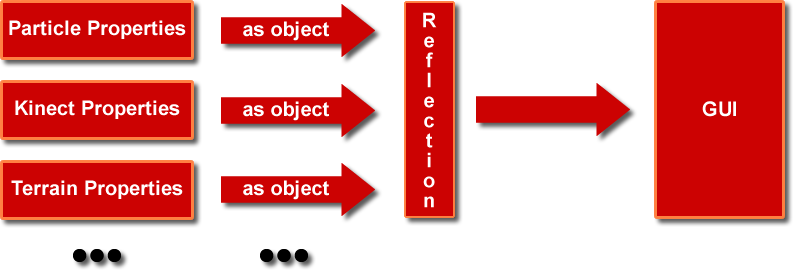
\includegraphics[width=280px]{graphics/GUIReflect.png}	
	\caption{Dynamische Konstruktion des GUI.}
	\label{fig:GUIReflect}
\end{figure}
	
\end{description}

\subsection{Das Ergebnis}
Auch bei dem GUI hat sich die Entscheidung für eine komplette Neuimplementierung ausgezahlt. Letztendlich entstand ein hoch flexibles, an den Windows 8 Stil erinnerndes (s. Abbildung \ref{fig:NewGui}) und durch unterschiedliche \textit{Themes} anpassbares (s. Abbildung \ref{fig:GUIThemes}) GUI System, welches uns viel Arbeit beim Hinzufügen von Bedienelementen einsparte und die Gesamtleistung unseres System, durch den \textit{Single-Window} Ansatz, nahezu verdoppelte.

\begin{figure}[h!]
	\centering
	\vspace*{10px}
	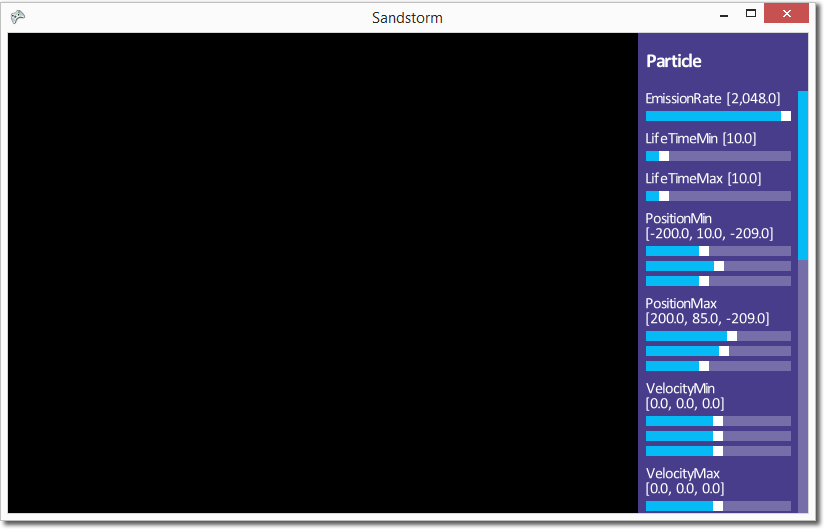
\includegraphics[width=\columnwidth]{graphics/newGui2.png}
	\caption{Das neue ingame GUI.}
	\label{fig:NewGui}
\end{figure}

\begin{figure}[h!]
	\centering
	\vspace*{10px}
	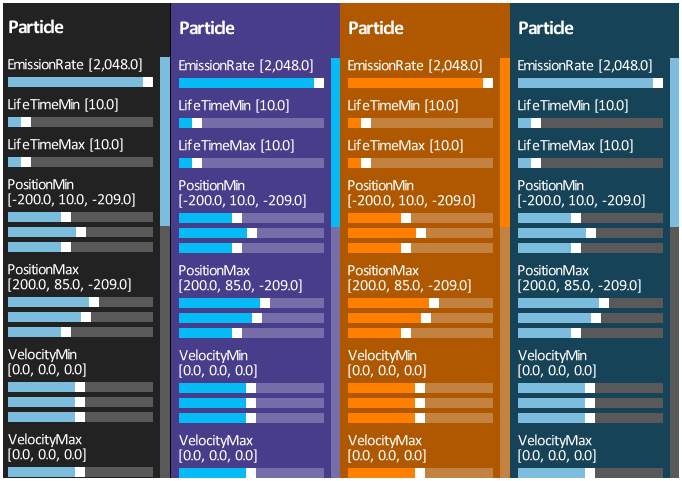
\includegraphics[width=290px]{graphics/guiThemes.png}
	\caption{Unterschiedliche Erscheinungsbilder des GUI.}
	\label{fig:GUIThemes}
\end{figure}

\end{Spacing}
\newpage

\clearpage
%% End Of Doc